

In this chapter we present some background related to creating a multi-media data repository. There are two main approaches: capturing data manually often by human annotating it, and automatic capturing. Automatic may or may not have a substep where a human has to filter/annotate the data. 


\section{Types of analyse}

In soccer there are several phases where you use analytic to help you gain insight. 

\subsection{Prematch}

Pre-match you use analytic to find weaknesses in the opponents team, on individually bases or the team as whole. You look at your team matched up against your opponent. A typical situation is that the manager gets an video summary of the opponent highlighting the opponents strengths and weaknesses. The video summary is often made up by the coaching staff who may use tools like Interplay. 

Typically in TV you have pundits bringing you analytic of key battles during the build up to the game. 


\subsubsection{In match}

During match the coaching staff continuously analysis the match and makes adjustment. Of course it is the players who makes all the decisions in the end, but the coach is the boss and most of the time players listen to what hes says. An adjustment to the formation can potentially be the tipping point in the game.

Tromsø IL uses a system NAME INSERT that lets you annotate sequences of a game with entity's like player, comment. This information will then be time synchronized with the video feed. Later, like in the break or in the game even, you can search on entity's to get the  corresponding video feed. As the system is available on an tablets players can in the middle of the match come to sideline to see a involvement. It can be anything that is tagged like a player involvement to a team move.

Using data gathered from sports data company like Opta you can get statistics live during the game. Its popular in TV to show statistics like ball possession percent, how far players have run or passes played to mention a few. 

\subsubsection{Post match}

During the post match the coach team goes through the game to evaluate the team performance. This is valuable as you get very concrete information about good and bad.  

\section{Manually capturing }

\subsection{Opta }


One of the big players Opta uses manual input to create their data repository. They have editorial teams across the world that captures data manually for the most popular soccer leagues. For example to capture statistics for one match, 3 humans have to be involved to be able to annotate all data. The data is captured via an application specifically created for the purpose of capturing data as quick and easily as possible. The editorial teams of Opta need to be able to identify a player, registrate a pass his made or a tackle, in a very short time to be able to keep up with the pace of the game. They study things like which shoe color a player has to be able to quickly identify the player.

Opta capture all types of actions like passes, type of pass, attacks, and interceptions. For each action they log they add a series of description tags like pitch coordinate, player, team and time-stamp. For every single pass they registrate if it was a through ball, normal ball or even a headed flick on from a long ball. For shots they registrate the foot it was kicked with, if it was a volley and so on . All this is done while the match is playing. About 1600 individual events are recorded in a standard match. 

\begin{lstlisting}
<Event id="290575408" event_id="5" type_id="1" period_id="1" 
min="0" sec="5" player_id="20856" team_id="810" outcome="1" 
x="44.6"y="61.1" timestamp="2007-08-12T13:00:24.827" 
last_modified="2007-08-12T13:00:25">
<Q id="1774596260" qualifier_id="141" value="91.6"/>
<Q id="1429253465" qualifier_id="140" value="49.9"/>
<Q id="1084400575" qualifier_id="56" value="Back"/>
</Event>
\end{lstlisting}

Here is an example of an event registrated in the Opta database. The event has a series of qualifiers describing it. Except from the obvious as timestamp and last modified dates we see that the player id, team id, time of event, x and y coordinates and the outcome of the event are registrated. Also we see that some extra details are included. In this example it maps to a pass from [44.6, 61.1] to [91.6, 49.9].

\begin{lstlisting}
<Q id="1774596260" qualifier_id="coordX" value="91.6"/>
<Q id="1429253465" qualifier_id="coordY" value="49.9"/>
<Q id="1084400575" qualifier_id="56" value="Back"/>
\end{lstlisting}


\subsubsection{PROZONE/AMISCO}
PROZONE3  is another system that tries to track players. Their data capture system incorporates 8-12 cameras, which is strategically positioned throughout the stadium so it covers 100 percent of the ground with some redundancy in case of a faulty component. They also incoperate the TV-camera feed, which obivously always follows the ball. All cameras are hooked into one server and uploaded at the end of the game before sent to undertake the tracking process. 

\begin{figure}[ht!]
\centering
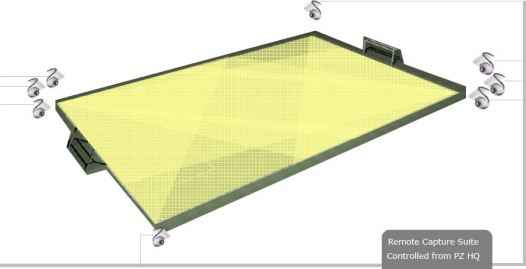
\includegraphics[width=150mm]{images/general/prozonecam.png}
\caption{The PROZONE camera system illustrated}
\label{overflow}
\end{figure}

The coding and tracking process of the players movement and actions is a manual process at present time. The process of knowing where every players is and doing is still to be seen done by a software completely alone without human guiding. There is a large department dedicated for post processing the game. With the help of the many cameras with different camera angles the team track players and on the ball events. Events and players gets an positional tag by using the pitch dimensions and coordinates. As different football grounds houses different pitch sizes the pitch dimensions has to be taken into account by calibrating the cameras (ASK SIMON). How do you know how far a player has run? This is calculated from the events and notating where players has run combined with the known pitch size and coordinates. The whole input process is done in a own software which helps you minimize the amount of manual work. The software follows rules created by basic machine learning algorithms to validate and verify the input. A simple example would be if the ball goes out of play the system will now that the next event will be a throw in, corner kick or goal kick \cite{Prozone:indepth}.

They claim to be able to track every movements of every player on the pitch every 10th of a second without using 3 any physical equipment on the players. When it comes to accuracy Di Salvo et al. [7] conducted an empirical evaluation of deployed ProZone systems at Old Trafford in Manchester and Reebook Stadium in Bolton, and concluded that the video camera deployment gives an accurate and valid motion analysis. The data is after a match available through the PROZONE3 interface. 


\subsection{Automatic capturing}
SAP places sensors in shin guards, clothing, and in footballs. The data can be applied to individual and team movement profiles to track distances, speed averages, ball possession, player tendencies and more . 

A similar system is the ZXY sport trackingsystem. The system is in used by premier league soccer teams in Norway, including Tromsø IL. Data captured is stored in Sybase databases with each match requiring about 500-700MB storage  The players have to wear a belt around their waist for the system to work. The ZXY system is able to track the player’s movement very detailed with an accuracy of 0.5m. It has a resolution of 20 samples per second. It relies on a radio-based signaling substrate to provide real-time high-precision positional tracking, including acceleration and heart rate. The home arena for Tromsø IL, Alfheim, is currently equipped with 10 receivers . A receiver tracks an specific area of the soccer field and combined they cover the whole pitch with some redundancy areas. The communication from the belt to the receivers goes on a 2.45-5.2 G Hz frequency radio signal. To compute the positional data the stationary radio receiver uses an advance vector based processing of the received radio signal. The data is aggregated and stored into a relational database.

Including the positions of the players the ZXY also gives you the step frequency and speed. 

\subsection{Wrap up}
The main problem with tracking systems that uses physical sensors is that usually only one of the teams wears the sensors.  This limits the functionality of the system as a opponent analysis system. You only get data for one team. 

On the other hand you have the manually systems that requires some human annotation. These system are able to track both teams. As they rely on human annotation of some degree they get more rich data as well. This includes pass type, key-passes, tackles, interceptions and so on. 

\begin{figure}[ht!]
\centering
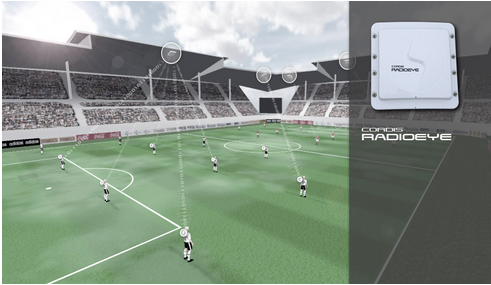
\includegraphics[width=150mm]{images/general/zxyoverview.png}
\caption{The PROZONE software - individual player analysis gives you statistics of performance over time}
\label{overflow}
\end{figure}


\subsubsection{Sensor based}


\subsection{Presenting data}

Most presenting of data is based around single matches. Figure 2.2 shows an example of how FourFourTwo presents data from a match. They use statistics from Opta. 

\subsubsection{Prozone}


PROZONE comes with several softwares to illustrate the data. The most relevant is the opposition analysis system. 

2D animation
Single player analysis
Team analysis
Pressing analysis
Success/direction
Player tempo
Passing movements
Receving the ball
Player events

\begin{figure}[ht!]
\centering
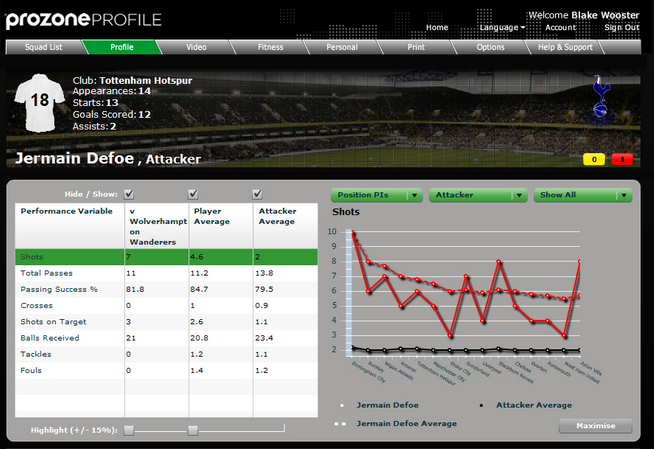
\includegraphics[width=100mm]{images/general/prozonestats.png}
\caption{The PROZONE software - individual player analysis gives you statistics of performance over time}
\label{overflow}
\end{figure}

On individual level you can get basic tactics like shots, total passes, passing success, crosses, shots on target, balls received, tackles, fouls. 

Doing queries on the data can give you all sprints for a certain player. Players in certain areas of the field have more intensive sprints when they first are involved thus are more vulnerable to injuries. Knowing the actual physical load on players can prevent injuries by regulating the training intensity and amount of time on each exercise.

\subsubsection{ZXY}
  
ZXY provides you with a 3D graphic interface. This interface lets you see the players action in real time by reading the data stream to reproduce the players action. The data is streamed in real time into the database as the match goes on. While watching you can produce timestamps of different events and produce manual input which is time synchronized with the automatic data. Naturally you can build your own software on top of the Sybase database. Tromsø IL in collaboration with University of Tromsø has made several systems to complement the ZXY software. Muithu and Bagadus.

\begin{figure}[ht!]
\centering
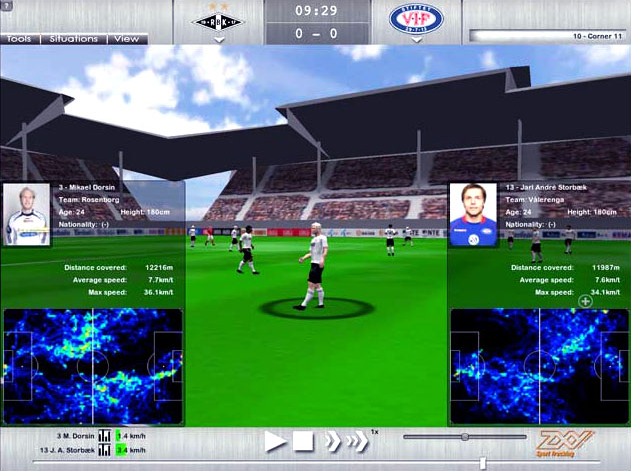
\includegraphics[width=100mm]{images/general/zxysoftware.png}
\caption{The ZXY software - tracking of players gives you information of distance covered, average speed and max speed. You also get a heat map of the players movement on the field.}
\label{overflow}
\end{figure}

\cite{dailymailOnStatistics}
